% =============================================
% Part 0.0 编辑个人信息
% =============================================

\newcommand{\department}{计算机系}		%在这里修改系别
\newcommand{\major}{大数据}				%在这里修改专业
\newcommand{\class}{大数据1701}					%在这里修改班级
\newcommand{\name}{	张丹颖		}			%在这里修改姓名
\newcommand{\stuid}{ 	2017011760		}				%在这里修改学号
\newcommand{\newdate}{	2018-11-21		}				%在这里修改日期 yyyy-mm-dd
\newcommand{\loc}{	实验室		}					%在这里修改地点

% =============================================
% Part 0.1 编辑课程信息
% =============================================
\newcommand{\newcourse} {数据结构\LARGE{(C)}} %在这里修改成课程名称
\newcommand{\newtitle}{ 二叉树的生成与操作} %在这里修改实验项目
\newcommand{\exptype}{计算机}

\newcommand{\grades}{}
\newcommand{\group}{无}

\newcommand{\tutor}{丁濛}
\newcommand{\onespace}{\hspace{1em} }
\begin{document}
\begin{titlepage}
	\centering
	\vspace*{1cm}
	{\fontsize{34pt}\baselineskip 实\onespace 验\onespace 报\onespace 告}\\
	\vspace{2cm}
	\fontsize{19pt}\baselineskip
	\makebox[30mm]{课程名称:}
	\underline{\makebox[75mm][c] {\newcourse} }
	\vskip 0.3cm
	\makebox[30mm]{实验项目:}
	\underline{\makebox[75mm][c] {\newtitle }}\\
	\vskip 0.3cm
	\makebox[30mm]{实验仪器:}
	\underline{\makebox[75mm][c]{ }}\\%在这里修改实验仪器
	\vskip 1cm

    \begin{table}[!htbp]
      \centering
      \sihao
      \begin{tabular}{| c | c | c | c | c | c |}
      	\hline
        项目 & 报告格式 & 写作质量 & 逻辑、注释质量、思想描述 & 复杂度分析 & 合计\\
        \hline
        
        百分比(\%) & 15 & 25 & 40 & 20  & 100 \\
        \hline
        得分	& {\gradeFormat } & {\gradeCode } & {\gradeComment}   & {\gradeComplex} & {\gradeTotal} \\
        \hline
      \end{tabular}
    \end{table}
     \Comments
    	
	\vskip 2cm

        \begin{table}[!tbhp]
            \centering
            \sanhao
            \begin{tabular}{ll}
                系\hspace{2em}别:	&	 \underline {\makebox[60mm][c]	{\department} 	} \\
                专\hspace{2em}业:	&	 \underline {\makebox[60mm][c] {\major}		} \\
                班级姓名:		&	\underline {\makebox[60mm][c] {\class\ \name\ }		} \\
                日\hspace{2em}期:	&	 \underline {\makebox[60mm][c]	{\newdate} 	} \\
                成\hspace{2em}绩:	&	 \underline {\makebox[60mm][c] {\grades}		} \\
                同组成员:		&	\underline {\makebox[60mm][c] {\group}		} \\
                指导教师:		&	\underline {\makebox[60mm][c] {\tutor}		} \\
            \end{tabular}
        \end{table}


%    
%    

\end{titlepage}

\newpage
% =============================================
% Part 2 Main document
% =============================================
\xiaosihao
\section{实验目的}
\begin{enumerate}
\item 掌握二叉树的链式存储结构;
\item 验证二叉树的前续、中序、后序(递归方式)以及层序的遍历;(验证)
\item 验证二叉树的中序遍历(非递归方式的实现以及不用栈的实现);(验证)
\item 验证二叉搜索树的插入、查找操作以及这些操作的复杂度和树高之间的关系;(验证)
\item 实现一个霍夫曼编码或实现一棵AVL树。(设计、综合)
\end{enumerate}

\section{实验内容}
\subsection{项目一}
实现以链表形式存储的二叉树,要求具有如下功能:
\begin{enumerate}
\item 构造,析构;
\item 递归版的前序遍历、中序遍历、后序遍历;
\item 层序遍历;
\item 通过用户输入(层序完全二叉树形式),建立一棵二叉树。用户输入以字符串的形式给出,其中'$\#$'表示空节点。
\end{enumerate}

\subsection{项目二}
改造第一题中的二叉树存储节点形式,使其支持能以非递归且不用额外栈的形式进行中序遍历。


\subsection{项目三}
在第二题的基础上,实现一棵二叉搜索树(Binary Search Tree),要求提供以下功能:
\begin{enumerate}
\item 向树中插入一个元素;
\item 前序、中序遍历一棵BST;
\item 查找某个元素。
\end{enumerate}

编写测试用例测试你的程序,验证BST树的查找和树高的关系。

\subsection{项目四}
实现一个霍夫曼编码(在平台上完成)。(4, 5任选一道即可)
\begin{enumerate}
\item 用户提供待编码的字符以及每个字符的频度,你给出编码结果。注意:构造霍夫曼树时,左儿子的频度应小于右儿子的频度;编码时,左儿子的前缀码为0,右儿子的前缀码为1。
\item 得到每个字符的编码后,输入一组由给定字符组成的明文,给出其对应的编码结果;
\item  然后对于编码结果,根据编码规则,写出其对应的明文。
\end{enumerate}

\subsection{项目五}
实现一棵AVL树(在平台上完成)。实现一棵AVL树,支持一个一个向树中加入元素,前序以及中序遍历AVL树的功能;支持查找AVL是否包含某个元素的功能。测试你的AVL树和BST树,在同样数据下的查找效率。


\section{实验过程}
\subsection{项目1}
大致思想 blablabla
\subsubsection{实验步骤}
\subsubsection{必要代码}
\lstinputlisting[language=C++]{code/main.cpp}
\subsubsection{实验结果}
	\begin{figure}[!bthp]
	\centering
        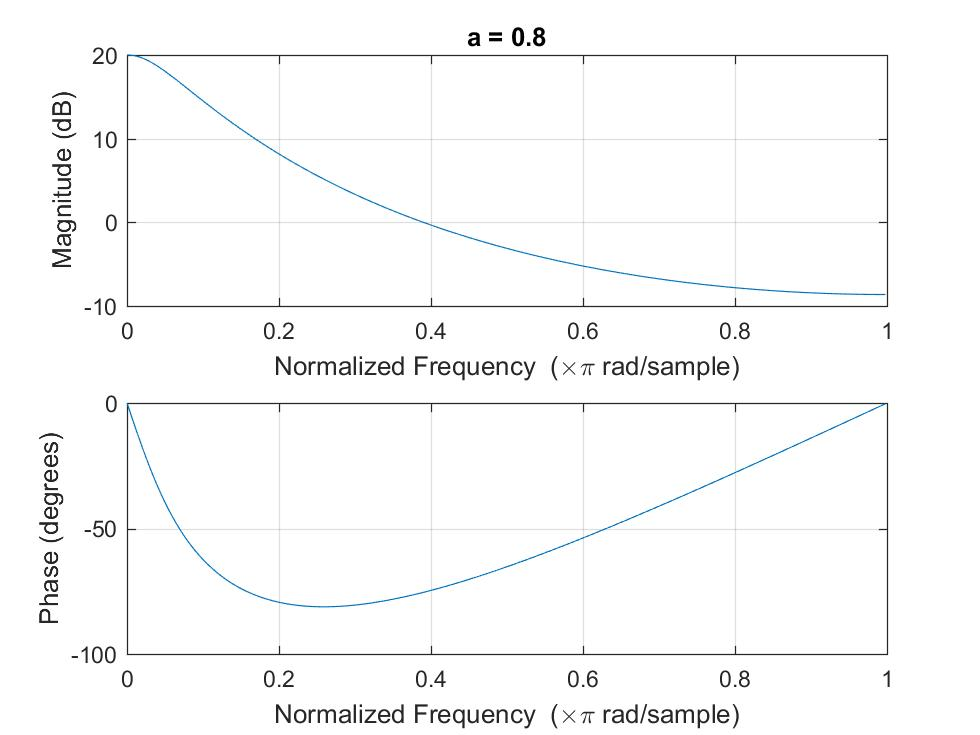
\includegraphics[width=0.6\linewidth]{02-1.jpg}
        \caption{D大调}
      \end{figure}

\subsection{项目2}
大致思想 blablabla sdfhasdfklj asd flas jkfjaksdf asd f
fasdf aksdjf klasj dfa
sdf
asdf

f
\subsubsection{实验步骤}
\subsubsection{必要代码}
\subsubsection{实验结果}

\subsection{项目3}
大致思想 blablabla
\subsubsection{实验步骤}
\subsubsection{必要代码}
\subsubsection{实验结果}

\subsection{项目4}

\section{实验总结}

\end{document}
